\documentclass[11pt,a4paper]{article}
\usepackage{solutions}
\usepackage{pgfplots}
\pgfplotsset{compat=1.18}
\usetikzlibrary{arrows.meta}
\newcommand{\vv}[1]{\vec{#1}}
\begin{document}
\doctitle{Physics A}{PC track \,$\cdot$\, Paper no.~3 \,$\cdot$\, Tuesday 14 April 2026}
         {4 hours, no calculator}{Worked solutions}

\begin{remark}
Questions refer to the English translation in this folder (\texttt{physics-a-pc\_paper\_en.pdf}),
which keeps the numbering of the original French paper. Notation: $\varepsilon_0$ is the
vacuum permittivity, $k_B$ the Boltzmann constant, $e$ the elementary charge.
\end{remark}

%==========================================================================
\partheading{Part I --- Electrospray ionisation}
\subpart{Parallel-plate capacitor}

\question{1}
Neglecting edge effects, the field between the plates is uniform and perpendicular to them.
It points from the positive plate to the negative one, and outside the capacitor it vanishes.
By Gauss's theorem (or Coulomb's theorem at the surface of a conductor):
\begin{result}
$E = \dfrac{\sigma}{\varepsilon_0}$, \quad where $\sigma$ is the surface charge density of the
positive plate.
\end{result}

\question{2}
The electrostatic energy per unit volume is $u_e = \dfrac{\varepsilon_0E^2}{2}$.

\question{3}
Consider an isolated capacitor (charges $\pm Q$ fixed) with plate area $S$ and gap $x$.
Since $E = \sigma/\varepsilon_0$ does not depend on $x$, the stored energy is
$W = u_e\,Sx = \frac{\varepsilon_0E^2}{2}Sx$. Move one plate by $\dd x$ at constant charge.
The electric force $F_x$ on that plate does the work $F_x\,\dd x = -\dd W$, so
$F_x = -\frac{\varepsilon_0E^2}{2}S < 0$: the plates attract. Per unit area,
\begin{result}
$P = \dfrac{\varepsilon_0E^2}{2} = \dfrac{\sigma^2}{2\varepsilon_0}$, directed towards the
other plate.
\end{result}
Equivalently, the force pulls the surface of each conductor \emph{outwards}, along its outward
normal and into the region where the field is. It acts like a negative pressure, whatever the
sign of $\sigma$.

Check: the surface charges feel the average of the fields on either side of the plate,
$\frac12(0 + \sigma/\varepsilon_0)$, so the force per unit area is
$\sigma\cdot\frac{\sigma}{2\varepsilon_0}$.

\subpart{Charged spherical drop; Rayleigh stability criterion}

\question{4}
In a conductor at equilibrium the charge sits on the surface, with $\sigma = \frac{Q}{4\pi R^2}$.
By spherical symmetry and Gauss's theorem,
$\vv E(r) = \frac{Q}{4\pi\varepsilon_0r^2}\,\vv e_r$ for $r > R$, and $\vv E = \vv 0$ inside.
At the surface $E = \frac{Q}{4\pi\varepsilon_0R^2} = \frac\sigma{\varepsilon_0}$, so
\begin{result}
$P = \dfrac{\varepsilon_0E^2}{2} = \dfrac{Q^2}{32\pi^2\varepsilon_0R^4}$, normal to the surface
and directed outwards.
\end{result}

\question{5}
The electrostatic force per unit area (outwards) beats the cohesive force per unit area
(inwards) when
$\dfrac{Q^2}{32\pi^2\varepsilon_0R^4} > \dfrac\gamma R$, that is,
\begin{result}
$|Q| > Q_{\lim} = 4\pi\sqrt{2\varepsilon_0\gamma R^3}$.
\end{result}
With the true Laplace pressure $2\gamma/R$ of a sphere, the same balance gives Rayleigh's limit
$8\pi\sqrt{\varepsilon_0\gamma R^3}$, larger by a factor $\sqrt2$ (footnote~1). Note that
$Q_{\lim}\propto R^{3/2}$. A drop that evaporates at constant charge therefore eventually
reaches the limit and breaks up.

\subpart{Taylor cone}

\question{6}
Outside the cone there is no charge, so the potential obeys Laplace's equation, $\Delta V = 0$.
The liquid is a conductor at equilibrium, so its surface is an equipotential: $V = V_0$ (the
potential of the capillary) on the whole cone $\theta = \theta_0$.

\question{7}
At every point, the electrostatic pull $\frac{\varepsilon_0E^2}2$ must balance the surface
tension $\propto\gamma/r$. So $E^2\propto1/r$, that is,
\begin{result}
$E \propto r^{-1/2}$.
\end{result}

\question{8}
With $V = V_0 + r^\delta f(\theta)$, the field $\vv E = -\vv\nabla V$ has components
$E_r = -\delta r^{\delta-1}f(\theta)$ and $E_\theta = -r^{\delta-1}f'(\theta)$, so
$|\vv E|\propto r^{\delta-1}$. Question~7 requires $\delta - 1 = -\frac12$:
\begin{result}
$\delta = \frac12$.
\end{result}

\question{9}
The problem is symmetric under rotation about the axis, so $V$ does not depend on $\phi$. In
spherical coordinates,
$\Delta V = \frac1{r^2}\partial_r(r^2\partial_rV) + \frac1{r^2\sin\theta}\partial_\theta(\sin\theta\,\partial_\theta V)$.
The radial part turns $r^{1/2}$ into $\frac12\cdot\frac32\,r^{-3/2}$, and the angular part
gives $r^{-3/2}$ times derivatives of $f$. So $\Delta V = r^{-3/2}\,[\dots]$, where the bracket
depends on $\theta$ only. The power of $r$ factors out (separation of variables), leaving a
\emph{linear second-order ordinary differential equation} for $f(\theta)$: second order because
the Laplacian is. (For reference: $f'' + \cot\theta\,f' + \frac34f = 0$, Legendre's equation
with index $\frac12$.)

\question{10}
On the cone, $V = V_0$ for every $r$, so $r^{1/2}f(\theta_0) = 0$ for all $r$:
\begin{result}
$f(\theta_0) = 0$.
\end{result}
Together with regularity on the jet axis $\theta = 0$, this selects
$f\propto P_{1/2}(\cos\theta)$. Its first zero is $\theta_0\simeq130.7^\circ$, i.e.\ a
half-angle $\pi - \theta_0\simeq49.3^\circ$ for the liquid cone (the ``Taylor angle''). We
checked this value numerically.

\question{11}
By Coulomb's theorem, just outside the liquid $\sigma = \varepsilon_0E\propto r^{-1/2}$. The
surface charge density therefore \emph{grows without bound towards the apex}: the charge
concentrates at the tip, where the field is also strongest. The jet that leaves the tip
carries matter with a very large charge per unit volume, so the small droplets it breaks into
are highly charged, close to the Rayleigh limit. As they evaporate, $R$ decreases at constant
$Q$ while $Q_{\lim}\propto R^{3/2}$ decreases. They reach the limit again and split
repeatedly, finally producing multiply charged ions.

%==========================================================================
\partheading{Part II --- Ion cyclotron resonance mass spectrometry}

\question{12}
Newton's law with the Lorentz force,
$m\frac{\dd\vv v}{\dd t} = q(\vv E + \vv v\times\vv B)$, can be written
$\frac{\dd\vv v}{\dd t} = \frac qm(\vv E + \vv v\times\vv B)$. The equation, and hence the
trajectory for given initial conditions, only involves $q/m$. Two ions with the same $m/q$
follow the same trajectory, so the motion gives access to $m/q$, not to $m$.

\question{13}
Electric charge is quantised: it is carried by electrons and protons, each of charge $\mp e$.
An ion formed by removing $z$ electrons (or adding $z$ protons) carries $q = ze$ with $z$ a
positive integer.

For two neighbouring peaks of the same molecule, with charges $z$ and $z+1$,
$p_z = m/z$ and $p_{z+1} = m/(z+1)$. Then $p_z - p_{z+1} = \frac{m}{z(z+1)} = \frac{p_{z+1}}{z}$, so
\[
  z = \frac{p_{z+1}}{p_z - p_{z+1}} .
\]
\begin{itemize}
\item Peak at $1999.30$, with its neighbour $1888.29$: $z = \frac{1888.29}{111.01}\simeq17.0$,
  so $z = 17$.
\item Peak at $1000.15$, with its neighbour $971.54$: $z = \frac{971.54}{28.61}\simeq34.0$, so
  $z = 34$.
\end{itemize}
Consistency check: $1999.30/1000.15\simeq2 = 34/17$. The 16 peaks in between are
$z = 18,\dots,33$; the one for $z = 32$, near $m/z\simeq1063$, is visible but unlabelled.
Then $m = 17\times1999.30\simeq3.399\times10^4$~u and $m = 34\times1000.15\simeq3.401\times10^4$~u:
\begin{result}
$m\simeq3.40\times10^4$~u, i.e.\ about 34~kDa.
\end{result}
Every labelled peak of the series agrees. Each gives an integer $z$ (to $\pm0.1$) and a value
of $z\times(m/z)$ between 33\,983 and 34\,006~u:
\begin{center}\small
\begin{tabular}{c|ccccccccc}
$z$ & 15 & 17 & 19 & 21 & 24 & 27 & 30 & 34 & 36\\ \hline
$m/z$ & 2265.52 & 1999.30 & 1788.93 & 1618.60 & 1416.43 & 1259.16 & 1133.33 & 1000.15 & 944.61\\
$z\,(m/z)$ & 33\,983 & 33\,988 & 33\,990 & 33\,991 & 33\,994 & 33\,997 & 34\,000 & 34\,005 & 34\,006
\end{tabular}
\end{center}
\begin{remark}
The slow drift of $z\,(m/z)$ with $z$ reveals that the ions are really $[M+z\mathrm H]^{z+}$:
each charge comes with a proton ($1.007$~u). Subtracting it,
$M = z\,(m/z - 1.007)$ gives $33\,970\pm2$~u for \emph{all} the peaks. That is a relative
precision of $10^{-4}$, which illustrates why the method is so accurate.
\end{remark}

\emph{Number of atoms.} A protein contains H (1~u), C (12~u), N (14~u), O (16~u) and a little
S (32~u). Roughly half of its atoms are hydrogen, so the mean mass per atom is about 7~u. (For
example, an amino-acid residue weighs about 110~u for about 16 atoms.) Hence
\begin{result}
$N_{\text{atoms}}\sim\dfrac{3.4\times10^4}{7}\approx5\times10^3$ atoms: a few thousand atoms,
or about 300 amino acids.
\end{result}

\question{14}
A long solenoid (length much larger than its radius) with $n$ turns per unit length, carrying
a steady current $I$, produces inside it a uniform axial field $B = \mu_0nI$. To reach several
tesla ($B = 7$~T in question~42 requires $nI\approx5.6\times10^6$~A/m), the coil is
superconducting. Helmholtz coils are a simpler alternative for weak fields.

\question{15}
With $\vv v\times\vv B = B(\dot y,\,-\dot x,\,0)$:
\begin{result}
$m\ddot x = qB\,\dot y,\qquad m\ddot y = -qB\,\dot x,\qquad m\ddot z = 0.$
\end{result}

\question{16}
$\ddot Z = \ddot x + \ii\ddot y = \frac{qB}m(\dot y - \ii\dot x) = -\ii\frac{qB}m(\dot x + \ii\dot y)$,
so $\ddot Z = -\ii\frac{qB}{m}\dot Z$. Substituting $Z = Z_0\ee^{-\ii\omega_0t}$ gives
$-\omega_0^2Z = -\ii\frac{qB}m(-\ii\omega_0)Z = -\frac{qB}m\omega_0Z$, so, since
$\omega_0\neq0$,
\begin{result}
$\omega_0 = \dfrac{qB}{m}$ \quad (the cyclotron angular frequency).
\end{result}
\emph{Check} in real coordinates. For $x = R\cos\omega_0t$ and $y = -R\sin\omega_0t$,
$m\ddot x = -mR\omega_0^2\cos\omega_0t$ and $qB\dot y = -qBR\omega_0\cos\omega_0t$. These are
equal if and only if $\omega_0 = qB/m$, and the same holds for the $y$ equation. For $q > 0$,
$Z\propto\ee^{-\ii\omega_0t}$ turns \emph{clockwise} when seen from $+z$, which is the known
sense of rotation of a positive charge about $\vv B$. The angular frequency does not depend on
the radius or the speed.

\subpart{Excitation}

\question{17}
$F_x + \ii F_y = F(\cos\omega t - \ii\sin\omega t) = F\ee^{-\ii\omega t}$, so
\begin{result}
$m\ddot Z = -\ii qB\dot Z + F\ee^{-\ii\omega t}$, \quad i.e.\ \quad
$\ddot Z + \ii\omega_0\dot Z = \dfrac Fm\ee^{-\ii\omega t}$.
\end{result}

\question{18}
$(m/\tau)v$ is a force, so $m/\tau$ is in kg\,s$^{-1}$ and \textbf{$\tau$ is a time}. Without
other forces, $\vv v$ would relax as $\ee^{-t/\tau}$. The same form appears in the
\textbf{Drude model} of electrical conduction, where an electron feels $-(m/\tau)\vv v$, with
$\tau$ the mean time between collisions; this gives $\sigma = ne^2\tau/m$. It also appears for
linear viscous friction (Stokes drag $-6\pi\eta R\,\vv v$, with $\tau = m/6\pi\eta R$).

\question{19}
$m\ddot Z = -\ii qB\dot Z - \frac m\tau\dot Z + F\ee^{-\ii\omega t}$, that is,
$\ddot Z + \left(\ii\omega_0 + \frac1\tau\right)\dot Z = \frac Fm\ee^{-\ii\omega t}$. With
$Z = Z_0\ee^{-\ii\omega t}$:
$\left[-\omega^2 + \omega_0\omega - \ii\frac\omega\tau\right]Z_0 = \frac Fm$, hence
\begin{result}
$Z_0 = \dfrac{F}{m\,\omega\,\left(\omega_0 - \omega - \dfrac{\ii}{\tau}\right)}.$
\end{result}

\question{20}
$|Z_0| = \dfrac{F}{m\omega\sqrt{(\omega-\omega_0)^2 + 1/\tau^2}}$. If friction is weak,
$\omega_0\tau\gg1$. Then the square root has a sharp minimum at $\omega = \omega_0$, over which
the factor $1/\omega$ hardly varies. So $|Z_0|$ has a sharp maximum (a resonance) at
$\omega\simeq\omega_0$, of height $|Z_0|_{\max}\simeq F\tau/(m\omega_0)$. It falls by a factor
$\sqrt2$ when $|\omega-\omega_0| = 1/\tau$, so the full width at half maximum of $|Z_0|^2$ is
\begin{result}
$\Delta\omega\simeq\dfrac2\tau\sim\dfrac1\tau$, \quad a quality factor
$\omega_0/\Delta\omega\sim\omega_0\tau\gg1$.
\end{result}
\begin{center}
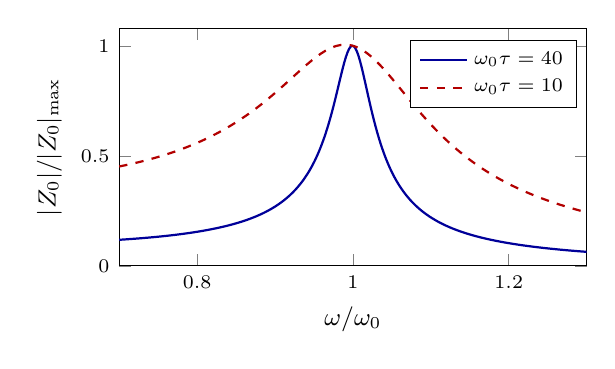
\begin{tikzpicture}
\begin{axis}[width=0.62\textwidth, height=4.6cm, xmin=0.7, xmax=1.3, ymin=0, ymax=1.08,
  xlabel={$\omega/\omega_0$}, ylabel={$|Z_0|/|Z_0|_{\max}$}, samples=300, domain=0.7:1.3,
  legend style={font=\scriptsize, at={(0.98,0.95)}, anchor=north east}, tick label style={font=\scriptsize},
  label style={font=\small}]
\addplot[thick, blue!60!black] {(1/x)/sqrt((x-1)^2+(1/40)^2)*(1/40)};
\addlegendentry{$\omega_0\tau = 40$}
\addplot[thick, dashed, red!70!black] {(1/x)/sqrt((x-1)^2+(1/10)^2)*(1/10)};
\addlegendentry{$\omega_0\tau = 10$}
\end{axis}
\end{tikzpicture}
\end{center}

\question{21}
Since $\omega_0 = zeB/m$, we have $m/z = eB/\omega_0$. Two ions with the same $z$ and masses $m$
and $m+\delta m$ resonate at frequencies differing by $\delta\omega_0 = \omega_0\,\delta m/m$.
They can be told apart only if $\delta\omega_0\gtrsim\Delta\omega\sim1/\tau$, i.e.
\[
  \frac{\delta m}{m}\gtrsim\frac1{\omega_0\tau} = \frac{m}{zeB\tau}.
\]
The width $\Delta\omega\sim1/\tau$ is set by collisions (and by the measurement time), not by
$z$ or $B$. Increasing $z$ and $B$ raises $\omega_0 = zeB/m$: the ions make more turns per
damping time, the relative line width shrinks, and closer masses can be resolved.

\question{22}
Here $F_x = qE\cos\omega t$ and $F_y = 0$, so
\[
  F_x + \ii F_y = qE\cos\omega t = \frac{qE}{2}\ee^{-\ii\omega t} + \frac{qE}{2}\ee^{-\ii(-\omega)t}.
\]
Each term has the form of question~17 with amplitude $F = qE/2$. The first (angular frequency
$+\omega$) rotates in the same sense as the ions. The second ($-\omega$) rotates the other way,
with $F_x = \frac{qE}2\cos\omega t$ and $F_y = +\frac{qE}2\sin\omega t$. The equation is linear,
so the forced motion is the sum of the two responses given by question~19:
\begin{result}
$Z(t) = \dfrac{qE/2}{m\omega(\omega_0 - \omega - \ii/\tau)}\,\ee^{-\ii\omega t}
      - \dfrac{qE/2}{m\omega(\omega_0 + \omega - \ii/\tau)}\,\ee^{+\ii\omega t}.$
\end{result}
For $\omega\simeq\omega_0$, the first amplitude is resonant ($\simeq qE\tau/2m\omega_0$). The
second has a denominator $\simeq2m\omega_0^2$ and is smaller by a factor
$\sim1/(2\omega_0\tau)\ll1$. \textbf{The co-rotating component} (angular frequency $+\omega$,
turning with the ions) causes the resonance. The counter-rotating one only produces a tiny
non-resonant wobble.

\question{23}
Use two parallel plane electrodes perpendicular to $x$, at $x = \pm d/2$, connected to a
sinusoidal voltage generator $u(t) = U\cos\omega t$. Between them, as in a plane capacitor,
$E_x = \frac Ud\cos\omega t$. The quasi-static approximation holds because $d\ll c/\omega$.

\question{24}
Keep only the resonant component ($F = qE/2$, $\omega = \omega_0$) and drop friction:
\begin{result}
$\ddot Z + \ii\omega_0\dot Z = \dfrac{qE}{2m}\,\ee^{-\ii\omega_0t}.$
\end{result}

\question{25}
With $Z = \ii At\,\ee^{-\ii\omega_0t}$: $\dot Z = (\ii A + A\omega_0t)\ee^{-\ii\omega_0t}$ and
$\ddot Z = (2A\omega_0 - \ii A\omega_0^2t)\ee^{-\ii\omega_0t}$, so
$\ddot Z + \ii\omega_0\dot Z = A\omega_0\,\ee^{-\ii\omega_0t}$. Identifying with question~24,
$A\omega_0 = \frac{qE}{2m}$:
\begin{result}
$A = \dfrac{qE}{2m\omega_0} = \dfrac{E}{2B}$ \quad (a velocity, the same for all ions).
\end{result}

\question{26}
$Z = \frac{Et}{2B}\,\ee^{\ii(\pi/2-\omega_0t)}$, so in polar coordinates
$r = \frac{Et}{2B}$ and $\theta = \frac\pi2 - \omega_0t$. Eliminating $t$:
\begin{result}
$r = \dfrac{E}{2B\omega_0}\left(\dfrac\pi2 - \theta\right)$: an \textbf{Archimedean spiral}
that starts at the origin and is travelled clockwise. Its radius grows by $\pi E/(B\omega_0)$
per turn.
\end{result}
\begin{center}
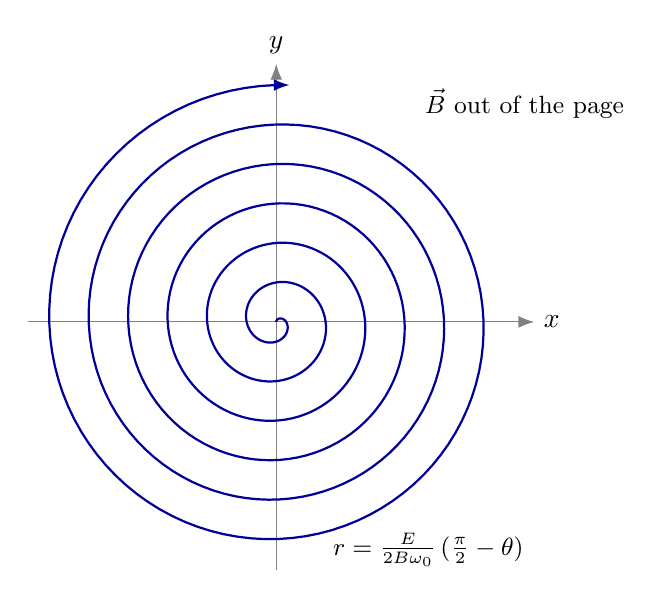
\begin{tikzpicture}[scale=0.42, >={Latex[length=2mm]}]
  \draw[->, gray] (-7.5,0) -- (7.8,0) node[right, black] {$x$};
  \draw[->, gray] (0,-7.5) -- (0,7.8) node[above, black] {$y$};
  \draw[thick, blue!60!black, domain=0:37.7, samples=600, variable=\t]
    plot ({0.19*\t*cos(deg(pi/2-\t))}, {0.19*\t*sin(deg(pi/2-\t))});
  \draw[->, thick, blue!60!black] ({0.19*37.7*cos(deg(pi/2-37.7))}, {0.19*37.7*sin(deg(pi/2-37.7))})
    -- ++({0.4*sin(deg(pi/2-37.7))}, {-0.4*cos(deg(pi/2-37.7))});
  \node[font=\small, anchor=west] at (4.2,6.6) {$\vv B$ out of the page};
  \node[font=\small] at (4.6,-6.9) {$r = \frac{E}{2B\omega_0}\,(\frac\pi2-\theta)$};
\end{tikzpicture}
\end{center}
\emph{Roles.} The magnetic field makes the ion turn at the cyclotron frequency $\omega_0$. Its
force is perpendicular to $\vv v$, so it does no work. At resonance, the co-rotating electric
force (of magnitude $qE/2$) turns together with the ion and keeps pushing along its velocity.
It feeds energy in steadily: $m\frac{\dd v}{\dd t} = \frac{qE}2$, so
$v = \frac{qE}{2m}t$ and $r = v/\omega_0 = \frac{E}{2B}t$, in agreement with question~25. The
speed and the radius grow linearly in time.

\question{27}
The radius $r(t) = \frac{Et}{2B}$ must become as large as possible without exceeding the cell
size, so $r(t_E)\sim d$:
\begin{result}
$t_E\sim\dfrac{2Bd}{E}\sim\dfrac{Bd}{E}$.
\end{result}
If the field is applied for longer, the ions hit the walls; if for less time, the signal
(question~40) is weaker.

\question{28}
The \textbf{uniformity of $\vv B$} matters more. The quantity measured is the frequency
$\omega_0 = qB/m$. A variation $\delta B$ over the region explored by the ions shifts the
frequency by $\delta\omega_0/\omega_0 = \delta B/B$. This broadens the line, limits the mass
resolution ($\delta m/m\sim\delta B/B$) and pushes ions at different radii out of resonance. A
non-uniform $\vv E$ only changes how fast the ions gain energy (their amplitude), not their
frequency.

\question{29}
By equipartition, $\frac12m\langle v^2\rangle = \frac32k_BT$, so, up to a factor $\sqrt3$,
\begin{result}
$p\sim\sqrt{m\,k_BT}$.
\end{result}

\question{30}
The radius of a circular motion in $\vv B$ is $r = \frac{mv_\perp}{|q|B} = \frac{p_\perp}{|q|B}$,
so $r\sim\frac{\sqrt{mk_BT}}{qB}$. The condition $r\ll d$ becomes $\sqrt{mk_BT}\ll qBd$, i.e.
\begin{result}
$m\ll m_{\max} = \dfrac{(qBd)^2}{k_BT}$.
\end{result}
For example, $q = e$, $B = 7$~T, $d = 3$~cm and $T = 300$~K give
$m_{\max}\approx3\times10^{-19}$~kg $\approx2\times10^8$~u. This is no limitation for
proteins, especially since $m_{\max}\propto z^2$.

\subpart{Trapping}

\question{31}
The magnetic force $q\vv v\times\vv B$ has no component along $\vv B = B\vv e_z$, and the
excitation field lies in the $(x,y)$ plane. Nothing acts along $z$, so $\ddot z = 0$. An ion
entering with a (thermal) velocity $v_z$ drifts uniformly along $z$ and leaves the cell.

\question{32}
$\vv E = -\vv\nabla V = (\alpha x,\ \alpha y,\ -\alpha\beta z)$. The cell is free of charge, so
$\Delta V = \frac\alpha2(-2-2+2\beta) = 0$:
\begin{result}
$\beta = 2$, \quad $V = \frac\alpha2(2z^2 - x^2 - y^2)$, \quad
$\vv E = (\alpha x,\ \alpha y,\ -2\alpha z)$.
\end{result}

\question{33}
$m\ddot z = qE_z = -2q\alpha z$, so $\ddot z + \omega_p^2z = 0$ with
\begin{result}
$\omega_p = \sqrt{\dfrac{2q\alpha}{m}}$
\end{result}
(since $q\alpha > 0$): a harmonic oscillation about $z = 0$. The ions are now confined along
$z$.

\question{34}
In the plane, the trapping field adds the force $q\alpha(x,y)$. It is radial and points
\emph{outwards}: a potential that confines along $z$ must repel in the plane, because
$\Delta V = 0$ (Earnshaw's theorem). Since $q\alpha/m = \omega_p^2/2$,
\begin{result}
$m\ddot Z = -\ii qB\dot Z + q\alpha Z$, \quad i.e.\ \quad
$\ddot Z + \ii\omega_0\dot Z - \dfrac{\omega_p^2}{2}Z = 0$.
\end{result}

\question{35}
With $Z = Z_0\ee^{-\ii\omega t}$: $-\omega^2 + \omega_0\omega - \frac{\omega_p^2}2 = 0$, i.e.
$\omega^2 - \omega_0\omega + \frac{\omega_p^2}2 = 0$. The discriminant
$\omega_0^2 - 2\omega_p^2$ is positive because $\omega_p\ll\omega_0$, so there are two real
roots:
\[
  \omega_\pm = \frac{\omega_0\pm\sqrt{\omega_0^2 - 2\omega_p^2}}{2},
  \qquad \omega_+ + \omega_- = \omega_0,\quad \omega_+\omega_- = \frac{\omega_p^2}2 .
\]
Using $\sqrt{\omega_0^2-2\omega_p^2}\simeq\omega_0 - \omega_p^2/\omega_0$:
\begin{result}
$\omega_+\simeq\omega_0 - \dfrac{\omega_p^2}{2\omega_0}$, \qquad
$\omega_-\simeq\dfrac{\omega_p^2}{2\omega_0}$.
\end{result}

\question{36}
The in-plane motion is a superposition of two circular motions,
$Z = Z_+\ee^{-\ii\omega_+t} + Z_-\ee^{-\ii\omega_-t}$.
\begin{itemize}
\item The fast one, at $\omega_+$, is the cyclotron motion, slightly shifted: its relative
  shift is $\frac{\omega_0-\omega_+}{\omega_0}\simeq\frac{\omega_p^2}{2\omega_0^2}\ll1$. The
  resonance frequency is only slightly modified (and the shift can be corrected for).
\item The slow one (the ``magnetron'' motion) has
  $\omega_-\simeq\dfrac{\omega_p^2}{2\omega_0} = \dfrac{2q\alpha/m}{2qB/m} = \dfrac\alpha B$.
  This is \textbf{independent of $m/q$}, and $\omega_-/\omega_0\simeq\omega_p^2/2\omega_0^2\ll1$.
\end{itemize}
Physically, the slow motion is the $\vv E\times\vv B$ drift in the radial field $E_r = \alpha r$.
The drift speed is $\alpha r/B$, hence the angular velocity $\alpha/B$, the same for every ion.

\subpart{Detection}

\question{37}
$V_i = \displaystyle\sum_{j\ne i}\frac{q_j}{4\pi\varepsilon_0\,|\vv r_i - \vv r_j|}$.

\question{38}
With $r_{ij} = |\vv r_i-\vv r_j| = r_{ji}$,
\[
  \sum_iq_iV'_i = \sum_i\sum_{j\ne i}\frac{q_i\,q'_j}{4\pi\varepsilon_0r_{ij}}
  = \sum_j\sum_{i\ne j}\frac{q_j\,q'_i}{4\pi\varepsilon_0r_{ji}}
  = \sum_iq'_i\sum_{j\ne i}\frac{q_j}{4\pi\varepsilon_0r_{ij}} = \sum_iq'_iV_i .
\]
The middle step just renames the dummy indices $i\leftrightarrow j$; the last step uses the
symmetry $r_{ij} = r_{ji}$.

\question{39}
With no charge between the plates, held at $\mp V/2$ and with $S\gg d^2$, the configuration is
a plane capacitor. The field is uniform and the potential is linear in $y$:
$V'(y) = Vy/d$ (equal to $-V/2$ at $y = -d/2$ and to $+V/2$ at $y = d/2$). Hence
\begin{result}
$V'_0 = \dfrac{V\,y_0}{d}$.
\end{result}

\question{40}
The actual configuration has $q_0 = q$ and $V_1 = V_2 = 0$; the auxiliary one has $q'_0 = 0$,
$V'_1 = -V/2$, $V'_2 = V/2$ and $V'_0 = Vy_0/d$. Reciprocity gives
$q_0V'_0 + q_1V'_1 + q_2V'_2 = q'_0V_0 + q'_1V_1 + q'_2V_2$, whose right-hand side is $0$.
So $q\frac{Vy_0}{d} + \frac V2(q_2-q_1) = 0$:
\begin{result}
$\Delta q = q_2 - q_1 = -\dfrac{2q\,y_0}{d}$.
\end{result}
Check: when the ion touches electrode~2 ($y_0\to d/2$), $\Delta q\to-q$, and electrode~2 carries
the whole image charge $-q$.

\emph{Detection of the resonance.} After the excitation, the ions of a given $m/z$ turn
together (coherently) on a circle of radius $r$ at $\omega_+\simeq\omega_0$. So
$y_0(t) = r\sin(\omega_+t+\varphi)$ and $\Delta q(t) = -\frac{2qr}{d}\sin(\omega_+t+\varphi)$.
Charge sloshes from one plate to the other through the connecting wire. This \emph{image
current} $i = \frac12\frac{\dd\Delta q}{\dd t}$ oscillates at the angular frequency of the ions.
Measuring its frequency gives $\omega_0 = qB/m$, hence $m/q$. Its amplitude, proportional to
$qr/d$, is why a large orbit is needed (question~27).

\question{41}
The two faces perpendicular to $x$ already carry the excitation electrodes (question~23), and
the $z$ faces carry the trapping electrodes. Using the $y$ faces for detection separates
excitation from detection. By symmetry, the excitation field $E_x$ induces no charge
difference between the $y$ plates, so the detection circuit does not pick up the huge
excitation signal and sees only the motion of the ions. (Since the orbit is circular, the
signal would be as strong along $x$ as along $y$.)

\question{42}
The highest frequency in the signal belongs to the smallest $m/z$ in figure~2,
$(m/z)_{\min}\approx900$ (in u). Since $\omega_0 = zeB/m = \frac{e}{m_u}\,\frac{B}{(m/z)}$,
\[
  f_{\max} = \frac{\omega_0}{2\pi} = \frac{10^8\times7}{2\pi\times900}\approx\frac{7\times10^8}{5.7\times10^3}
  \approx1.2\times10^5\ \mathrm{Hz}.
\]
By the Nyquist--Shannon criterion, the sampling frequency must exceed twice the highest
frequency present:
\begin{result}
$f_{s,\min} = 2f_{\max}\approx2.5\times10^5$~Hz (about 250~kHz).
\end{result}
Taking the left edge of the axis, $m/z\approx850$, gives about $2.6\times10^5$~Hz: the same
order of magnitude.

\question{43}
The detected signal is proportional to the charge of the ion: $\Delta q = -2qy_0/d\propto z$.
Moreover $\omega_0\propto z$, so the image current $i\propto q\,\omega_0r/d$ grows like $z^2$.
Highly charged ions therefore give a much larger signal and a better signal-to-noise ratio, so
fewer ions are needed. (They also raise $m_{\max}\propto q^2$ in question~30, so heavy
molecules can still be excited efficiently.)

\par\vspace{8mm}
\begin{center}\small\color{black!55}
Unofficial worked solutions. The questions are those of the X--ESPCI 2026 Physics~A paper
(PC track); the original French paper and its English translation are in this folder.
\end{center}
\end{document}
